%%
%% This is file `mcmthesis-demo.tex',
%% generated with the docstrip utility.
%%
%% The original source files were:
%%
%% mcmthesis.dtx  (with options: `demo')
%% 
%% -----------------------------------
%% This is a generated file.
%% 
%% Copyright (C) 2010 -- 2015 by latexstudio
%%       2014 -- 2019 by Liam Huang
%%       2019 -- present by latexstudio.net
%% 
%% This work may be distributed and/or modified under the
%% conditions of the LaTeX Project Public License, either version 1.3
%% of this license or (at your option) any later version.
%% The latest version of this license is in
%%   http://www.latex-project.org/lppl.txt
%% and version 1.3 or later is part of all distributions of LaTeX
%% version 2005/12/01 or later.
%% 
%% The Current Maintainer of this work is latexstudio.net.
%% 
%% !Mode:: "TeX:UTF-8"
%\documentclass{mcmthesis}
\PassOptionsToPackage{table}{xcolor}
\documentclass[
  CTeX = true,
  tcn = 2623614
]{mcmthesis}  % 当使用 CTeX 套装时请注释上一行使用该行的设置
\mcmsetup{tstyle=\color{black}\bfseries,%修改题号，队号的颜色和加粗显示，黑色可以修改为 black
        tcn = 2623614, problem = B, %修改队号，参赛题号
        sheet = true, titleinsheet = true, keywordsinsheet = true,
        titlepage = false, abstract = true}

\renewcommand{\team}{Team 2623614}

\geometry{
  left=1.8cm,
  right=1.8cm,
  top=2.0cm,
  bottom=1.8cm
}
    
% !TeX program = xelatex
\usepackage{fontspec}

\setlength{\parindent}{0pt}
\setlength{\parskip}{0.4em}

\newfontfamily\letterfont{Apple Chancery}

  %四款字体可以选择
  %\usepackage{times}
  %\usepackage{newtxtext}
  %\usepackage{palatino}
\usepackage{lastpage}
% ===== 中文支持（macOS + XeLaTeX）=====
\usepackage{fontspec}
\usepackage{xeCJK}

% 西文字体
\setmainfont{Times New Roman}

% 中文字体（macOS 自带）
\setCJKmainfont{Songti SC}      % 宋体
\setCJKsansfont{Heiti SC}       % 黑体
\setCJKmonofont{PingFang SC}   % 等宽

\xeCJKsetup{
  CJKmath = true
}
\usepackage{placeins}
\usepackage{graphicx}
%\usepackage[table]{xcolor}

\usepackage{indentfirst}  %首行缩进，注释掉，首行就不再缩进。
\newcolumntype{C}{>{\centering\arraybackslash}X}
\newcolumntype{M}[1]{>{\centering\arraybackslash}m{#1}}

\title{Decision-making Model for Combined Transportation System of Lunar Colonies Based on Pareto Optimization}


\author{}
\date{}



\linespread{1.0}
\setlength{\parskip}{1.2pt}
\begin{document}
\pagestyle{main}
\fancyhead[L]{\small\bfseries Team \# 2623614}
%\fancyhead[L]{\small\bfseries\itshape\leftmark}
%\fancyhead[R]{\small\bfseries\itshape Page~\thepage~of~\pageref{LastPage}}


\begin{abstract}
\setlength{\parindent}{2em}
\indent As lunar colonization programs transition into the phase of substantive construction, the development of an efficient, economical, and environmentally sustainable Earth-Moon logistics framework has emerged as a critical challenge. Aiming at the objective of establishing a lunar colony for 100,000 residents by 2050, this paper constructs a series of multi-dimensional coupled mathematical models to address the transport of 100 million tons of infrastructure materials, adaptation to non-ideal operating conditions, annual water resource replenishment, and Earth’s atmospheric environmental constraints.

\indent Regarding \textbf{Problem I}, a Hybrid Capacity Trade-off Optimization model based on Pareto optimality (HCTO-PM) was developed. By incorporating Wright's Law, the model establishes a dynamic cost iteration mechanism to quantitatively compare the space elevator (Option A), traditional rockets (Option B), and hybrid transportation (Option C). The results indicate that the hybrid approach performs optimally on the "time-cost" Pareto frontier: under a balanced decision-making strategy, completing the infrastructure mission requires 77 years at a total cost of approximately \$11.5 trillion.

\indent Regarding \textbf{Problem II}, a fault quantification and correction model was established. Considering stochastic factors such as cable oscillations, equipment failure rates, and rocket launch failure rates (5\%), the Pareto frontier was recalculated. Sensitivity analysis based on the single-parameter local perturbation method demonstrates that the pure elevator scheme exhibits the highest sensitivity to schedule fluctuations (with a 30.7\% duration extension), whereas the hybrid scheme demonstrates superior engineering resilience and risk mitigation through the synergistic effect of "fixed orbits plus discrete backups."

\indent Regarding \textbf{Problem III}, a Dynamic Mass Balance (DMS) model was constructed. By integrating data from human metabolism, Controlled Ecological Life Support Systems (BLSS), industrial oxygen production, and technical leakage, the net annual water resource deficit for a 100,000-person colony was calculated to be 35.4 kilotonnes. A comparison of replenishment pathways identifies the "elevator-primary with rocket-elastic-backup" mode as the optimal strategy, which reduces annual operating expenditures by approximately 14.2\% compared to pure rocket replenishment.

\indent Regarding \textbf{Problem IV}, this paper defines an Environmental Impact Unit (EIU) based on the Life Cycle Assessment (LCA) methodology. Utilizing the theory of stratospheric aerosol steady-state loading, it physically derives a threshold of 4,000 annual rocket launches as the maximum safety limit for Earth's atmosphere. By embedding this hard constraint into the optimization model, a three-dimensional Pareto mapping of "Time-Cost-Environment" was generated. The research proves that maximizing the utilization of space elevators is the only viable path for Earth's ecosystem to sustain the transport of 100 million tons of materials between the Earth and the Moon.

\indent Finally, a comprehensive policy recommendation letter was submitted to the MCM organization, covering site selection strategies, In-Situ Resource Utilization (ISRU), and dynamic scheduling mechanisms.
\begin{keywords}
Pareto multi-objective optimization; Wright's Law; Life Cycle Assessment; Space Elevator
\end{keywords}
\end{abstract}

\maketitle
\tableofcontents
\newpage
\section{Introduction}
\setlength{\parindent}{2em}
\subsection{Background} % 背景
\indent As the earth's resources become increasingly scarce and the population continues to grow, human civilization is facing unprecedented sustainable development challenges. As the closest celestial body to the earth, the moon is rich in helium-3, titanium, iron and other mineral resources, as well as its strategic value as a springboard for deep space exploration. It is a key target for international space agencies to compete for layout.

\indent However, traditional space transportation systems using rocket transportation have significant bottlenecks. Currently, according to SpaceX data, the cost of sending a 1 kilogram payload into low-Earth orbit is about US\$2,720, and the cost of reaching the lunar surface is even higher. This high-cost, low-frequency transportation mode severely restricts the construction of large-scale space infrastructure. At the same time, this solution also seriously affects the earth's ecological environment due to the harmful gas emissions produced by the fuel.

\indent In contrast, the space elevator system has shown breakthrough potential as a revolutionary space transportation infrastructure. The system uses the balance between the centrifugal force of the Earth's rotation and gravity to set a vertex anchor point in the geosynchronous orbit 35,786 kilometers above the equator, and connects to ground ports through a 100,000-kilometer-long super-strong material tether to form a "space highway." Compared with traditional rockets, space elevators use electricity as a power source and can theoretically achieve large-scale material transportation with nearly zero carbon emissions, reducing unit transportation costs to less than one thousandth of traditional methods.

\indent This topic focuses on the envisaged plan to colonize the moon with 100,000 people in 2050. It analyzes the time cycle and economic cost of transportation of engineering materials in the early stages of lunar base construction, and the different transportation options that can be adopted for the water demand of the base after residents move in. Then, it comprehensively considers the environmental impact of different transportation options and provides different transportation options.

%\subsection{Literature Review} % 文献综述


\subsection{Restatement of the Problem} % 问题重述

\textbf{Problem1}:
It is estimated that the construction of a lunar colony of 100,000 people will require 100 million tons of materials. Under ideal conditions (no rocket launch failure, no tether shaking), three different options are adopted:
\begin{itemize}
  \item a:Three galactic ports using only space elevators
  \item b:Traditional solution using only ten Earth rocket launch systems
  \item c:A combination of two transport systems
\end{itemize}

This article will establish a mathematical model to calculate the transportation costs and time required for these three different options.

\textbf{Problem2}:
Expand the model of Question 1 to consider the impact of non-ideal factors on the transportation plan, that is, consider factors such as cable shaking of the space elevator system, elevator damage, and launch failure factors of the rocket transportation system. Due to these non-ideal factors, the annual carrying capacity of both transportation systems, as well as the unit transportation costs, will be affected. These effects are combined in the model of Question 1 to obtain the adjusted transportation plan.

\textbf{Problem3}:
After the lunar colony is completed and operated, what is the total water demand for a population of 100,000 and its distribution? A mathematical model is established to analyze this problem. Combined with the transportation system model of questions 1 and 2, a water delivery plan with optimal additional costs and timing is obtained on the premise of ensuring water supply for the colony.

\textbf{Problem 4:}
During the process of transporting materials, launching rockets will inevitably have an impact on the earth's environment. However, the earth's environment can only bear limited pollution. This impact will be taken into consideration in the model to re-formulate the material and water resources transportation plan for the realization of a 100,000-person lunar colony base.


\subsection{The Description of the Problem} % 问题描述

\textbf{Problem1}:
The scene in question 1 is set against the background of the initial construction of the lunar colony. Humanity has built a complete space elevator system, which can transport supplies to the moon through the Galaxy Port, and can also use ground rocket launch systems to transport supplies to the lunar base. Under the assumption that both the rocket launch and the space elevator system work under ideal conditions (no capacity loss, no additional cost), three transportation options are used: three galactic ports relying only on the space elevator system, traditional rocket launch using only existing bases, or a combination of the two methods. The time and economic costs required for different options are modeled and analyzed. Among them, in the combination scheme of the two methods, in order to solve the comprehensive optimization of time and economy and analyze the rocket launch arrangement, the multi-objective Pareto optimization model can be used for analysis. 
At the same time, considering the possible decline in rocket manufacturing costs, the annual decay coefficient of rocket manufacturing is introduced based on Wright's law, and a rocket cost iteration model is added to Plan C to optimize the plan.

\textbf{Problem2}:
The ideal assumption of Question 1 ignores the inherent risks of the space transportation system: the ultra-long cable of the space elevator is affected by orbital disturbance and mechanical wear, and there are problems such as cable shaking and equipment failure; traditional rocket launches are affected by weather and technical complexity, and face risks such as launch failure and reduced launch site efficiency. Such non-ideal factors will directly lead to capacity attenuation, cost increase and construction period extension. It is necessary to quantify the impact of faults and correct the original model to ensure that the solution has reliability and anti-interference capabilities in actual engineering scenarios. 
Abstract faults can be converted into quantifiable coefficient indicators to build capacity attenuation and cost addition models. Embed non-ideal parameters into the multi-objective optimization model of Problem 1, recalculate the time and cost of the three types of options, generate the modified Pareto front, and obtain the adjustments of each option under non-ideal conditions.

\textbf{Problem3}:
The total water demand after the 100,000-person lunar colony completes operations can be based on existing data from the International Space Station (ISS), Biosphere 2, etc., and a per capita daily water flux model can be constructed based on scenarios. At the same time, in order to maximize the utilization of water resources, a water recycling system must be considered. Then, the water demand, recycling efficiency and loss rate of each scenario are integrated to calculate the annual net water resource deficit (i.e. the annual water resource demand of the base). Embed the net supply demand into the early transportation model, compare the costs, capacity matching, and long-term operation and maintenance resilience of the three types of transportation routes, and introduce the redundant design idea of ​​"main transportation + backup".

\textbf{Problem 4:}
Large-scale Earth-to-Moon transportation will have a cumulative impact on the Earth's environment. Among them, the source of pollution can be considered to be only the ground rocket launch system, while the space elevator system has zero emissions and no pollution during transportation. First, the environmental cost of the transportation solution needs to be quantified. A composite environmental impact equivalent can be constructed based on the life cycle assessment (LCA) method and the environmental damage weight of multiple types of pollutants can be integrated. Secondly, the earth's environmental pollution carrying threshold can be derived. Based on the stratospheric aerosol steady-state load theory, the maximum annual number of rocket launches that the earth can withstand can be physically derived. Finally, the environmental impact is regarded as the third goal, embedded in the original time-cost optimization model, using the atmospheric carrying capacity as a hard constraint, correcting the upper limit of rocket launch frequency, and screening the three-dimensional Pareto optimal solution.

\subsection{Our Work} % 我们的工作
\begin{figure}[htbp]
  \centering
  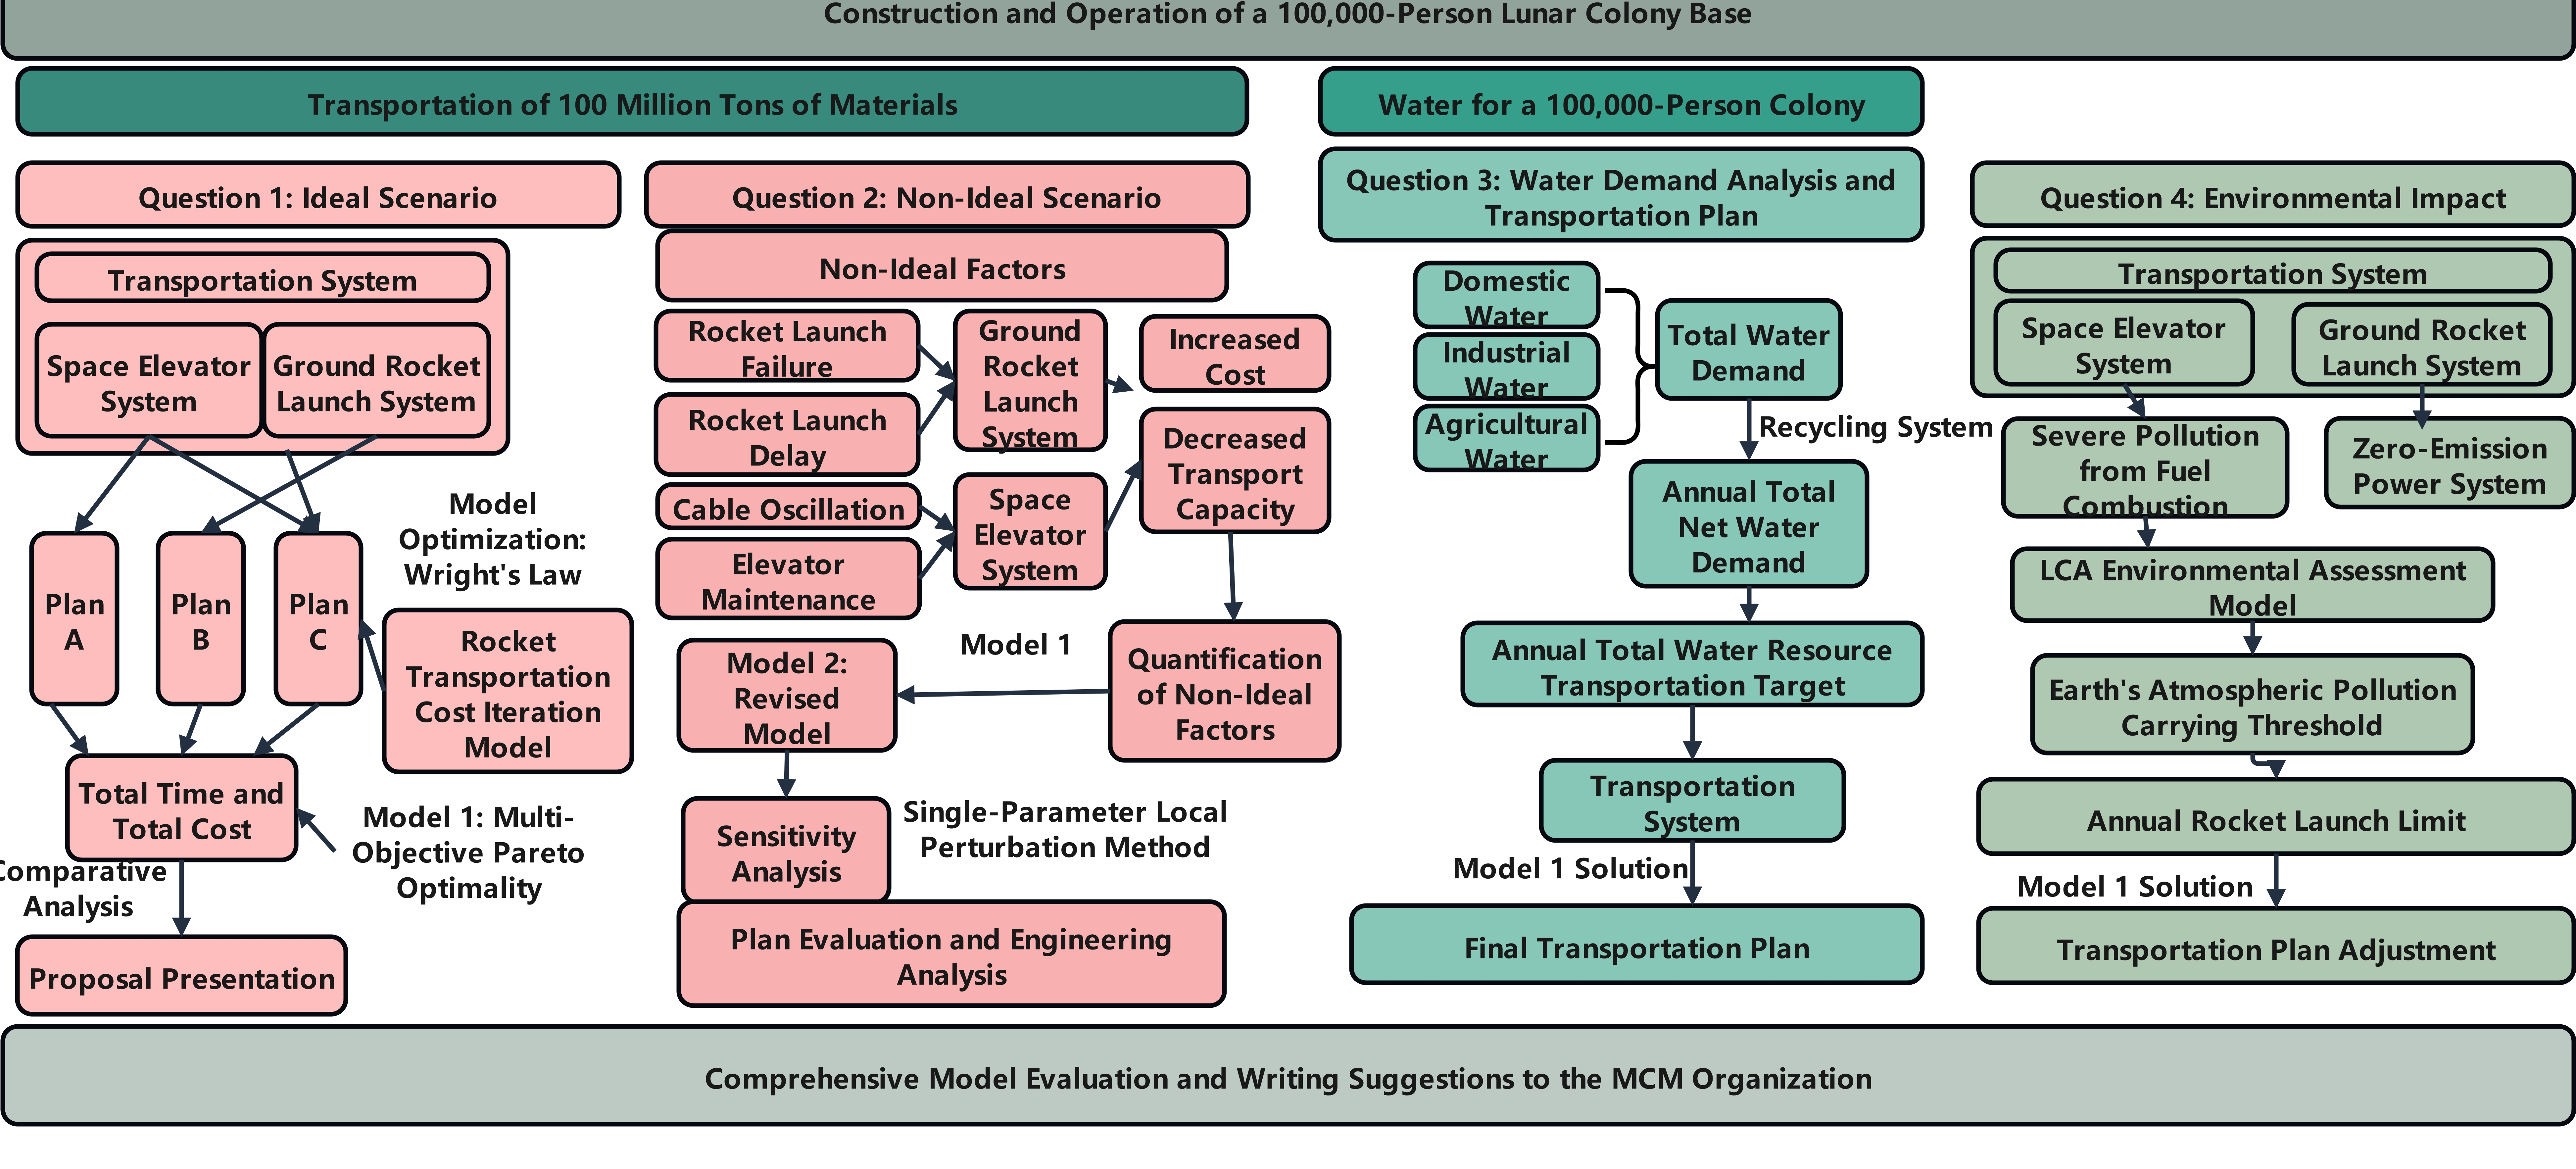
\includegraphics[width=1.00\textwidth]{../figures/ourwork.jpg}
  \caption{Our Work}
  \label{fig:Our Work}
\end{figure}
\FloatBarrier




\section{Assumptions}

\begin{enumerate}
\item
\textbf{Assumption:}  
The lunar base construction and material transportation process are planned with "year" as the basic time unit. 
Within a single year, transportation capacity, transportation costs and resource allocation strategies remain unchanged, and transportation decisions between different years are independent of each other.

\textbf{Justification:}  
This assumption is consistent with the industry practice of conducting overall planning on an annual cycle for large-scale aerospace projects.
By reasonably discretizing the time dimension, the model can focus on the core contradiction between transportation efficiency and cost while ensuring computational feasibility.
Furthermore, parameter variations between years can be characterized using a technology iteration model, thereby simplifying modeling complexity while maintaining scientific rigor and engineering feasibility.
\item
\textbf{Assumption:}  
The total amount of materials required for lunar base construction is determined at the beginning of modeling and does not change over time throughout the construction cycle. 
Additional material requirements due to design adjustments or unexpected needs are not considered in the model.

\textbf{Justification:}  
This assumption is consistent with the engineering practice of completing overall demand论证 and material planning for large-scale aerospace projects at the beginning of a mission.
By fixing the total material requirements, the model can effectively avoid uncertainty interference introduced by non-transportation factors, thereby focusing on analyzing the performance differences of different transportation schemes in terms of time and cost dimensions.

\item
\textbf{Assumption:}  
In normal operating conditions, the space elevator system has a clearly defined and stable annual maximum transportation capacity,
and its annual transportation volume does not exceed the system design upper limit, without considering short-term overloading operations.

\textbf{Justification:}  
This assumption is based on the fundamental principle of "safety first" in aerospace engineering and is consistent with the engineering characteristics of large-scale precision engineering systems operating under rated conditions.
The model directly adopts the technical parameters given in the problem statement as system capability constraints,thereby ensuring the reliability of model inputs and the engineering interpretability of results.

\item
\textbf{Assumption:}  
The annual availability rate of the space elevator system and the launch success rate of rockets are independent of each other across different years, and are not directly affected by historical operating conditions.

\textbf{Justification:}  
This assumption is based on the engineering characteristics that aerospace systems usually "reset" their operating status after annual maintenance and overhaul, effectively avoiding the modeling complexity caused by time dependence. 
At the same time, this processing method is consistent with the parameter settings given in the question, which helps to establish a unified and fair comparison benchmark between different transportation solutions.
\end{enumerate}

\newpage % Start notations on a new page
\section{Notations}
\setlength{\parindent}{2em} % 设置缩进为2个字符宽度

The core symbols and their definitions used in this study are summarized in Table~\ref{table:notations}, providing an overview of the key parameters and their related meanings.

\begin{table}[ht]
\centering % Center the table
\caption{Notations used in this literature}
\renewcommand{\arraystretch}{1.5}
\rowcolors{1}{gray!15}{white} % 从第1行开始，隔行灰色

\begin{tabular}{
>{\centering\bfseries\boldmath\arraybackslash}p{0.3\linewidth} |
>{\centering\arraybackslash}p{0.6\linewidth} 
}
\cline{1-2}
\textbf{Symbol} & \textbf{Description} \\ 
\cline{1-2}

$x$          & Number of rocket launches per year \\ \cline{1-2}
$M$          & Total mass to be transported to space (kilogram) \\ \cline{1-2}
$T$          & Time to complete the mission (years) \\ \cline{1-2}
$C_{total}$  & Total cost of the mission (dollar) \\ \cline{1-2}
$C_{SES}$    & Cost per kilogram of space elevator system (dollar/kg) \\ \cline{1-2}
$C_{launch}$ & Cost per kilogram of rocket launch (dollar/kg) \\ \cline{1-2}
$C_{total_0}$& Average total market transportation cost in the base year (current) \\ \cline{1-2}
$C_{fuel}$   & The theoretical fuel cost floor per 100kg of cargo \\ \cline{1-2}
$\alpha$     &The annual technology iteration decay factor for manufacturing and operating costs, with a value of 0.05 \\ \cline{1-2}
$P_{SES}$    & Annual throughput of the space elevator system (kilogram/year) \\ \cline{1-2}
$P_{launch}$ & Payload capacity per rocket launch (kilogram/launch) \\ \cline{1-2}
PSNR         & Peak signal-to-noise ratio for image quality evaluation \\ \cline{1-2}
UCIQE        & Underwater Color Image Quality Evaluation metric \\ \cline{1-2}
UIQM         & Underwater Image Quality Measure \\ \cline{1-2}

\end{tabular}
\label{table:notations}
\end{table}

%%%%%%%%%%%%%%%%%%%%%%%%%%%%%%%%%%%%%%%%%%%%%%%%%%%%%%%%%%%%%%%%%%%%%%%%%
%%%%%%%%%%%%%%%%%%%%%%%%%%%%%%%%%%%%%%%%%%%%%%%%%%%%%%%%%%%%%%%%%%%%%%%%%
%%%%%%%%%%%%%%%%%%%%%%%%%%%%%%%%%%%%%%%%%%%%%%%%%%%%%%%%%%%%%%%%%%%%%%%%%
%%%%%%%%%%%%%%%%%%%%%%%%%%%%%%%%%%%%%%%%%%%%%%%%%%%%%%%%%%%%%%%%%%%%%%%%%
%%%%%%%%%%%%%%%%%%%%%%%%%%%%%%%%%%%%%%%%%%%%%%%%%%%%%%%%%%%%%%%%%%%%%%%%%




\newpage % Start models on a new page
\section{Models}
\subsection{Modeling and Solving of Problem 1}

\subsubsection{Calculation of each scheme}
\paragraph{Scheme a: Only Space Elevator System}
\vspace{0.3em}
太空电梯系统由三个银河港组成，每个银河港每年可运输17.9万吨货物，$P_{SES} = 3 \times 179000 = 537000\ \mathrm{kg/year}$。
根据国际太空电梯协会（ISEC）的预测，太空电梯的运营成本可降至$C_{SES} = \$100/\mathrm{kg}$，这包含了电力消耗、维修及折旧等费用。
因此，仅使用太空电梯系统的时间为
\[T=\frac{M}{P_{SES}}\]
Total cost of the mission为
\[C_{total} = C_{SES} \times M \]
计算得出：仅使用太空电梯系统需要约186.22年，总成本约10万亿美元。

\paragraph{Scheme b: Only Rocket Launches}
\vspace{0.3em}
利用现有的十个发射场进行高频发射，每个火箭发射可携带$P_{launch} = 100000kg$的有效载荷，
单发火箭的成本为$C_{launch} = \$500/\mathrm{kg}$。
若设定目标工期为40年，则每年需要发射的火箭次数为
\[x = \frac{M}{P_{launch} \times T} \]
Total cost of the mission为
\[C_{total} = C_{launch} \times M \]
计算得出：若仅使用火箭发射且在40年完成，总成本约50万亿美元，但每年需要发射25000次火箭，日均发射约68次，
单个发射场在一天内需要发射约7次，远超当前全球发射能力，在工程上极其困难。

\paragraph{Scheme c: Combined Space Elevator and Rocket Launches}
\vspace{0.3em}
综合考虑太空电梯系统和火箭发射两种方法时，这是一个多目标优化问题，目标是最小化任务完成时间$T$和总成本$C_{total}$。
通过调整火箭发射次数$x$来达到两种方法的不同组合，从中找到时间和成本之间的平衡点。
%为刻画混合航天运输系统中任务时间与总成本之间的权衡关系，本文构建了一种混合运载能力权衡优化模型（HCTO-PM），并通过显式 Pareto 前沿进行决策分析。
To analyze the trade-off between mission completion time and total cost in a hybrid space transportation system,
a Hybrid Capacity Trade-off Optimization model with explicit Pareto Mapping (HCTO-PM) is developed.
该模型采用单参数控制的并行运输系统结构，决策变量$x$表示火箭的年发射次数，目标函数包括任务完成时间$T$和总成本$C_{total}$。
任务完成时间$T$由以下公式给出：
\[T = \frac{M}{P_{SES} + P_{launch} \times x} \]
总成本$C_{total}$由以下公式给出：
\[C_{\mathrm{total}}(x)=C_{SES}\cdot P_{SES}\cdot\frac{M}{P_{SES}+xP_{launch}}+C_{launch}\cdot P_{launch}\cdot x\]
Multi-Objective Formulation:
The model simultaneously considers the following two conflicting optimization objectives.
\[\begin{cases}
\min T(x)=\frac{M}{P_{\mathrm{SES}}+xP_{\mathrm{launch}}} \\
\min C(x)=C_{\mathrm{total}}(x) & 
\end{cases}\]
Without the assumption of explicit preference weights, this problem does not pursue a single optimal solution, 
but instead constructs a Pareto optimal solution set to characterize the efficiency boundary in the feasible decision space.
Since the model contains only one continuous decision variable, this paper uses the parameter sweep method to
perform high-resolution sampling of the feasible interval of $x$.
计算对应的时间–成本目标值，并通过非支配关系筛选得到 Pareto 前沿。
%\begin{figure}[htbp]
%    \centering
%    
\includegraphics[width=0.65\textwidth]{figures/pareto_scan.png}
%    \caption{时间–成本多目标优化问题的 Pareto 前沿}
%    \label{fig:pareto_scan}
%\end{figure}
%图~\ref{fig:pareto_scan}展示了时间–成本多目标优化问题的 Pareto 前沿。
从中选出部分关键解得到如下表格：
\begin{table}[htbp]
\centering
\caption{Trade-off Results under Different Rocket Launch Frequencies}
\label{tab:tradeoff_results}
\renewcommand{\arraystretch}{1.3}
\begin{tabular}{c c c}
\toprule
\textbf{Rocket Launches} $x$ (\textbf{times/year}) 
& \textbf{Completion Time} $T$ (\textbf{years}) 
& \textbf{Total Cost} $C$ (\textbf{million USD}) \\
\midrule
2{,}496  & 109.72 & 193{,}110.40 \\
4{,}997 & 77.72 & 378{,}986.12 \\
7{,}499 &49.09 & 752{,}636.23 \\
\bottomrule
\end{tabular}
\end{table}
根据不同的决策偏好可以从中选择适当的解决方案。
贴图

\subsubsection{Improvement of scheme c}
\paragraph{Rocket Iteration: Transportation cost iteration}
\vspace{0.3em}
理论基础:
在分析每 100kg 有效载荷的运输成本演变时，必须引入工业经济学中的核心概念——学习曲线模型（Learning Curve Model），
即莱特定律（Wright's Law）。该定律由 T.P. Wright 最早于 1936 年在航空制造领域提出，其核心论点表明：单位产品的生产成本
并不是随机波动的，而是随着累计产量的增加呈现出可预测的幂律下降趋势。在商业航天领域，这一效应被进一步修正为受“规模经济”与“复用频率”双重驱动的成本迭代机制。
在构建长周期的航天运输成本演变模型时，若仅采用单一的指数衰减模型，容易忽略物理化学层面的硬性约束。因此，本研究引入双因子成本结构（Dual-Factor Cost Structure），
将单次发射的单位质量成本  解构为两个性质迥异的组成部分：受工业学习曲线影响的箭体制造与运营成本$C_{body}$，以及受化学工业定价影响的相对刚性的燃料（推进剂）成本 $C_{fuel}$ 。
根据工业经济学中的莱特定律（Wright's Law），箭体制造与发射运营成本具有显著的“干中学”（Learning by Doing）特征，即随着累计发射量和复用次数的增加，该部分成本呈现幂律下降。
然而，燃料成本主要取决于液氧、甲烷或煤油的工业大宗商品价格，其波动受宏观能源市场影响，难以通过航天产业自身的规模效应实现数量级下降。因此，成本动力学方程应表达为：
\[C_{launch}=C_{man}(n)+C_{fuel}=C_1\cdot n^{-b}+C_{fixed}\]
其中，$n$ 为累计产出量，$b$ 为学习指数，而 $C_{fixed}$ 代表了由化学能密度决定的热力学成本底限。这一模型的引入，揭示了航天运输成本下降虽然在初期极其迅速，但在远期将逼近一个由物理极限决定的渐进值。
通过历史数据回溯可以发现，航天运输成本的结构正经历着从“硬件主导”向“能源主导”的范式转移。在传统航天飞机时代，每公斤约 54,500 美元的发射成本中，推进剂成本占比微乎其微（不足 0.1\%），绝大部分开支源于
一次性的硬件损耗与高昂的地面维护。此时，莱特定律对整体成本的削减作用极为显著。随着 SpaceX 猎鹰 9 号（Falcon 9）及星舰（Starship）架构的出现，高频复用技术彻底改变了这一比例。根据 ARK Invest 与
SpaceX 公开财务数据的交叉验证，猎鹰 9 号的燃料成本约为 20-30 万美元，仅占单次发射边际成本的极小比例，但在完全复用的星舰架构预期中，随着硬件均摊成本的急剧下降，燃料成本的占比将大幅提升。根据埃隆·马斯克
的工程预期，未来星舰的单次发射成本中，推进剂费用将成为主要的边际支出项。这表明，虽然制造成本可以通过 30\%-35\% 的高学习率（Learning Rate）快速摊薄，但燃料成本将构成一条不可逾越的水平渐近线（Horizontal Asymptote）。

参数设定:
为了构建适用于年度预测的数学模型，我们将基于“产量”的莱特定律映射为基于“时间”的年度衰减函数，并设定燃料成本为常量约束。假设全球航天发射频率维持当前的指数增长趋势，制造成本部分的年均优化效率将维持高位。
基于现有技术路径的分析，本模型设定如下核心参数：
- 制造成本衰减率：考虑到规模效应与复用技术的成熟，设定箭体制造与运营部分的年均衰减系数$\alpha$为 5\%。
- 燃料成本刚性：设定每 100kg 有效载荷分摊的燃料成本为常数$C_{fuel}$，作为成本演化的收敛极限。
综合考量，未来的单位运输成本将不再是无限趋近于零，而是沿着一条指数曲线逼近燃料成本底线。这种处理方式平抑了纯数学模型在远期预测中的失真风险，符合大规模物流网络的物理现实。

模型构建:
基于上述双因子分析，本研究建立每 100kg 货物运输成本$C_{launch}(t)$随时间$t$演变的最终迭代公式：
设$t$为年份(以模型起始年为$t = 0$)，$C_{launch}(t)$由可变动的制造部分$C_{man}(t)$和固定的燃料部分$C_{fuel}$，则有：
\[C_{launch}(t)=C_{man_0}\times(1-\alpha)^t+C_{fuel}\]
带入参数得：
\[C_{launch}(t)=(C_{total_0}-C_{fuel})\times(0.95)^t+C_{fuel}\]
该公式清晰地描述了成本下降的两个阶段：在近期（$t$较小时），由$(1 - \alpha)^t$主导，体现为成本的快速下降，符合摩尔定律般的指数特征；在远期（$t$趋于无穷大时）， $C_{launch}(t)$渐近收敛于 $C_{fuel}$，体现了能源价格对太空物流经济性的最终约束。

\paragraph{A new strategy based on the iterative models}
\vspace{0.3em}
基于上述迭代模型，我们提出了一种新的混合运输策略，以进一步优化运输成本与时间的权衡。在HCTO-PM模型的基础上，结合时间变量$t$引入动态成本调整机制来反映火箭发射成本随时间的演变，得到
Multi-Year Hybrid Capacity Trade-off Optimization with Pareto Mapping (MY-HCTO-PM)模型。该模型下的决策变量$x$不在是单一维度，而是会随着时间$t$动态调整的函数$x(t)$，以反映不同年份的发射频率选择。
优化目标函数同样包括任务完成时间$T$和总成本$C_{total}$，计算公式为
\[P_{SES}T+P_{launch}\cdot\sum_{t=0}^{T}x_{(t)} = M\]
\[C_{total}=C_{SES}\cdot P_{SES}\cdot T+\sum_{t=0}^{T}C_{launch}(t)\cdot x_{(t)}\cdot P_{launch}\]
对每个可行$T$, 求出用火箭发射的总运输质量后按年份倒序分配（从最后一年开始发射），以利用制造成本衰减优势。得到一组$(T,C)$ 数据点，即帕累托前沿。
为便于决策，定义三类代表性解：
- 均衡解（Balanced）：使用归一化后的时间和成本计算每个可行点到理想点 $(T_{min}, C_{min})$ 的欧氏距离，距离最小者即为均衡解
- 激进解（Faster）：均衡解向左偏移一定比例（减少总工期，允许成本增加）
- 经济解（Cheaper）：均衡解向右偏移一定比例（延长总工期以降低成本）
该方法保证了三类方案均落在最优折中区间内，可直观展示工期与成本之间的权衡关系。
% 贴图


\subsubsection{Conclusions of Problem}
太空电梯和传统火箭的组合更有利于实现高效且经济的太空运输。通过调整火箭发射频率，可以在任务完成时间和总成本之间找到最佳平衡点。
引入火箭运输成本的时间迭代模型后，提出了一种新的混合运输策略，进一步优化了运输方案。该策略通过动态调整火箭发射频率，利用制造成本的衰减优势，实现了更低的总成本和更短的任务时间。
基于MY-HCTO-PM模型，决策者可以根据不同的偏好选择均衡、激进或经济的运输方案，从而更好地满足实际需求。


\subsection{Modeling and Solving of Problem 2}
\subsubsection{Problem Analysis}


\subsubsection{Model Preparation}


\subsubsection{Model Construction}



\subsubsection{Model Solution}

% \input{../sections/5_Sensitivity_Analysis}
\section{Model Evaluation}

\subsection{Advantages}

The developed model system is systematic and forward-looking, characterized by the following three strengths:

\begin{enumerate}
    \item \textbf{Economic and Logistics Optimization:} The MY-HCTO-PM model transcends traditional single-objective optimization by integrating a ``two-factor cost structure'' and Wright's Law. This framework captures the physical trajectory of declining space transportation costs, avoiding the distortions of purely mathematical forecasting. Furthermore, Pareto Mapping provides practical decision-making trade-offs between mission cycles and budgetary constraints.
    \item \textbf{High-Precision Resource Management:} The water demand model for a lunar colony of 100,000 inhabitants accounts for complex fluxes—including physiological metabolism, ecological agriculture, industrial production, and technical losses such as airlock leakage. Validated against International Space Station (ISS) and closed-ecosystem experimental data, this multi-dimensional balance ensures a robust physical foundation for Earth-Moon logistics.
    \item \textbf{Innovative Sustainability Framework:} By incorporating Life Cycle Assessment (LCA) and stratospheric aerosol carrying capacity, the study introduces ``environmental cost'' as a third dimension to the time-cost trade-off system. This elevates the framework to a sustainable development model, quantitatively demonstrating the unique ecological advantages of space elevators for ultra-large-scale transportation.
\end{enumerate}

\subsection{Limitations}

Despite its performance, the model possesses certain limitations:

\begin{enumerate}
    \item \textbf{Linearity in Technology Iteration:} The model relies on historical parameters (e.g., 5\% annual decay), which may fail to capture the nonlinear, disruptive breakthroughs characteristic of aerospace technology. Sudden advancements in materials or propulsion (``black swan'' events) are difficult to account for within the current exponential decay framework.
    \item \textbf{Steady-State Assumptions:} The model simplifies the nonlinear coupling between lunar population growth and infrastructure expansion. By assuming a steady state post-construction, it may overlook the dynamic complexities of population migration and industrial ramping, potentially introducing biases during early expansion phases.
\end{enumerate}
\section{Letter of Advice}


{\letterfont
\noindent To: MCM Lunar Development Technical Committee

Subject: Technical Integration and Strategic Framework for the Development of a 100,000-Resident Lunar Colony

Dear Members of the Technical Committee,

In the context of the continuous advancement in aerospace engineering and deep-space exploration capabilities, the establishment of a lunar colony capable of supporting a permanent population of 100,000 has emerged as a tangible engineering challenge centered on systems engineering and the integration of critical technologies. Toward this objective, we propose the following recommendations from the perspectives of technical implementation and long-term operational sustainability.

Regarding Spatial Siting and Structural Design, the lunar south pole should be prioritized as the primary site. This region offers relatively stable illumination conditions and is rich in water ice resources within its Permanently Shadowed Regions (PSRs), which are essential for energy acquisition and life support. Residential and occupational zones should utilize modular, hermetically sealed, and semi-subterranean structures. By leveraging lunar regolith coverage for radiation shielding, thermal regulation, and micrometeoroid defense, the requirement for imported protective materials can be significantly reduced.

Regarding Life Support Systems, the colony must rely on a highly reliable closed-loop technological architecture. Water self-sufficiency can be achieved through ice mining and advanced wastewater treatment and recycling systems, aiming for a recovery rate of over 99%. The atmospheric system should integrate electrolysis for oxygen production, CO2 scrubbing, and photosynthetic processes. Food supply must be anchored by high-efficiency plant factories, algae cultivation, and synthetic food production to minimize reliance on terrestrial replenishment and enhance system security.

Energy Systems form the cornerstone of colonial operations. We recommend large-scale solar arrays as the primary energy source, supplemented by small-scale nuclear reactors for stability and emergency backup. Energy will not only sustain life support and habitats but also power industrial manufacturing, resource processing, and infrastructure expansion. This necessitates high-efficiency energy storage and intelligent distribution systems to mitigate the effects of the lunar diurnal cycle and sudden load fluctuations.

For Industrial and Infrastructure Construction, priority must be given to the development of In-Situ Resource Utilization (ISRU) technologies. Through the processing of lunar regolith, oxygen, metallic materials, and construction feedstock can be extracted for structural fabrication, equipment maintenance, and consumables production. This strategy will drastically lower long-term logistics costs and serves as the key technical pillar for large-scale, sustainable colonization.

At the Demographic and Social Operational level, population introduction should be phased, starting with scientific research, engineering, and medical personnel, followed by the gradual expansion of education, service, and administrative sectors. Comprehensive medical care, psychological support, and robust social organizational structures are as critical as technical systems for the stable survival of humans in long-term enclosed environments.

Finally, regarding Safety and Long-term Maintenance, the colony must incorporate multi-layered redundancy designs, including backup capacities for life support, energy supply, and communication systems. Systematic fault detection and emergency response mechanisms must be established to address equipment aging, environmental anomalies, and unforeseen risks.

In summary, the realization of a 100,000-person lunar colony depends on the mature integration of multiple key technologies rather than a single breakthrough. By steadily advancing resource utilization, energy security, and life support technologies, this goal remains feasible from an engineering perspective in the long term.

\begin{flushright}
Respectfully submitted,\\
Team 2623614
\end{flushright}
}
\begin{thebibliography}{99}


\bibitem{nasa_weather_07R}
National Aeronautics and Space Administration,
\emph{Launch Weather Guidelines (Weather-07R)},
NASA John F. Kennedy Space Center, FL, USA,
Available at: \url{https://www3.nasa.gov/centers/kennedy/pdf/167476main_Weather-07R.pdf},
Accessed: Feb.~2026.

\bibitem{water_electrolysis_2013}
Y.~Zhang, H.~Wang, and X.~Li,
\emph{Fundamental study of water electrolysis for life support system in space},
Electrochimica Acta,
2013, 100: 350--357,
doi:10.1016/j.electacta.2012.11.112.

\bibitem{adu2025water}
S.~Adu, W.~S.~Walker, and W.~A.~Jackson,
``Potable Water Recovery for Space Habitation Systems Using Hybrid Life Support Systems:
Biological Pretreatment Coupled with Reverse Osmosis for Humidity Condensate Recovery,''
\emph{Membranes}, vol.~15, no.~7, p.~212, Jul.~2025,
doi: 10.3390/membranes15070212.

\bibitem{nasa_iss_water_recovery}
National Aeronautics and Space Administration,
\emph{NASA Achieves Water Recovery Milestone on International Space Station},
NASA ISS Research Communications Team, June~20,~2023.
Available at: \url{https://www.nasa.gov/missions/station/iss-research/nasa-achieves-water-recovery-milestone-on-international-space-station/},
Accessed: Feb.~2026.

\bibitem{nelson2009water}
M. Nelson, W. F. Dempster, and J. P. Allen,
``The water cycle in closed ecological systems: Perspectives from the
Biosphere 2 and Laboratory Biosphere systems,''
\emph{Advances in Space Research},
2009.

\bibitem{vpk_moon_water_2024}
“Scientists have calculated the water supply for the lunar base for 100 people,” 
ВПК.name, June~3,~2024.
Available at: \url{https://vpk.name/en/870752_scientists-have-calculated-the-water-supply-for-the-lunar-base-for-100-people.html},
Accessed: Feb.~2026.

\bibitem{leger_oxygen_moon_2025}
D.~Leger, F.~Ghaffari-Tabrizi, M.~Shaw, J.~Rasera, D.~Dickson, B.~Valentin,
A.~Morlock, F.~Thoresen, and A.~Cowley,
``Modeling energy requirements for oxygen production on the Moon,''
\emph{Proceedings of the National Academy of Sciences of the United States of America},
vol.~122, no.~8, e2306146122, 2025.

\bibitem{abney_sabatier_h2}
M.~B.~Abney, L.~A.~Miller, and T.~Williams,
\emph{Sabatier Reactor System Integration with Microwave Plasma Methane Pyrolysis Post-Processor for Closed-Loop Hydrogen Recovery},
NASA Marshall Space Flight Center, Huntsville, AL, USA.

\bibitem{lpi_water_moon_2025}
Lunar and Planetary Institute,
\emph{Recent Study Assesses Strategies to Bring Back Water from the Moon},
LPI Features (Lunar and Planetary Institute), January~29,~2025.
Available at: \url{https://www.lpi.usra.edu/features/2025/012925/water-on-moon/},
Accessed: Feb.~2026.

\end{thebibliography}

%\input{../sections/9_Appendices}
%\AImatter

\begin{ReportAiUse}{9}
\bibitem{AI1}
Bing AI\\
Query1: Please help explain in detail what the Pareto Model is\\
Output: The Pareto Model, rooted in the Pareto Principle (commonly known as the 80/20 Rule), is a theoretical and 
analytical framework used to describe the skewed distribution of resources, effects, or outcomes in various natural, 
social, and economic systems. Named after Vilfredo Pareto, an Italian economist and sociologist who first documented 
this phenomenon in the late 19th century, the model has become a foundational tool for understanding imbalance and 
optimizing decision-making.
 ### Core Concept The central tenet of the Pareto Model is the **disproportionate relationship** 
between inputs and outputs: a small fraction of factors (typically around 20\%, called the "vital few") 
is responsible for a large majority of results (typically around 80\%, called the "trivial many"). 
Importantly, the 80/20 ratio is not a rigid mathematical constant but a heuristic—actual proportions may vary 
(e.g., 70/30, 90/10) depending on the context, but the underlying "skewness" remains consistent. For instance: 
- In wealth distribution, 20\% of a population might hold 80\% of a country’s total wealth; 
- In business operations, 20\% of a company’s products could generate 80\% of its revenue; 
- In quality management, 20\% of defect types may cause 80\% of production issues. 
### Mathematical Foundation: The Pareto Distribution The Pareto Model is mathematically formalized through 
the **Pareto Distribution**, a continuous probability distribution designed to characterize variables with a "heavy tail" 
i.e., a small number of extreme values and a large number of small values). 
Its key components include: 
1. **Probability Density Function (PDF)**: \[ f(x) = \begin{cases} \frac{\alpha x_0^\alpha}{x^{\alpha + 1}} & \text{for } x \geq x_0, \\ 0 & \text{for } x < x_0, \end{cases} \] - \( x \): 
The random variable (e.g., income, product sales, task impact);
 - \( x_0 \): The minimum value of \( x \) (scale parameter, representing the threshold below which no observations exist);
 - \( \alpha > 0 \): The shape parameter (Pareto index), which determines the degree of skewness—smaller \( \alpha \) means a more uneven distribution. 
2. **Cumulative Distribution Function (CDF)**: \[ F(x) = 1 - \left( \frac{x_0}{x} \right)^\alpha \quad \text{for } x \geq x_0, \] This function calculates the probability that \( x \) is 
less than or equal to a given value, illustrating how quickly the "vital few" dominate the distribution.
 ### Key Characteristics 
 1. **Unevenness**: Rejects the assumption of linear proportionality, emphasizing that outcomes are rarely distributed equally across factors. 
 2. **Scalability**: Applies across scales (from individual tasks to global systems) and domains (economics, business, engineering, etc.). 
 3. **Prioritization Focus**: Highlights the value of identifying and focusing on the "vital few" factors to maximize efficiency—allocating resources to these factors yields disproportionate returns.
 ### Practical Applications The Pareto Model’s simplicity and versatility make it widely used in diverse fields:
 - **Economics & Finance**: Analyzing income inequality, market concentration, and wealth distribution (e.g., measuring the Gini coefficient alongside Pareto metrics).
 - **Business Management**: Optimizing product portfolios (prioritizing high-revenue items), improving customer retention (focusing on high-value clients), and reducing operational waste (targeting key inefficiencies).
 - **Quality Control**: In lean manufacturing and Six Sigma, the "Pareto Chart" (a hybrid of bar chart and line graph) identifies the most frequent causes of defects, guiding process improvements. 
 - **Productivity & Project Management**: Prioritizing tasks to focus on high-impact activities, reducing time spent on low-value work, and allocating team resources effectively.
  ### Limitations
 - **Descriptive, Not Prescriptive**: The model describes *what is* (a skewed distribution) but not *why* it occurs or how to change it—it must be paired with causal analysis for actionable insights.
 - **Not Universal**: Not all phenomena follow a Pareto distribution; some systems (e.g., normal distributions in natural sciences) exhibit more balanced outcomes. 
 - **Risk of Oversimplification**: Overreliance on the 80/20 ratio may lead to neglecting the "trivial many," which could become critical over time (e.g., niche products that grow into major revenue streams). In essence, the Pareto Model is a powerful tool for recognizing imbalance, enabling individuals and organizations to prioritize effectively, optimize resource allocation, and achieve more with less by focusing on the factors that drive the most significant results.

\bibitem{AI2}
OpenAl Enie (Nov 5, 2023 version, Ernie 4.0)\\
Query1: What authoritative literatures are available on the technical principles, feasibility of space elevators, and their application in space colonization?\\
Output: The following literatures cover core aspects of space elevators (e.g., technical design, economic paradigm, deployment methods) and their integration with space colonization (e.g., Mars, Moon colonization), with sources including the International Space Elevator Consortium (ISEC), NASA, arXiv, and authoritative publishing platforms, ensuring academic rigor and practical reference value:
1. Literatures Focused on Space Elevator Fundamentals & Technical Feasibility

Title: Space Elevator: A Revolutionary Earth-to-Space Transportation SystemAuthors: Bradley Edwards, Eric WestlingPublisher/Year: BC Edwards Publishing, 2002Core Content: This book is a foundational work on space elevator technology. It systematically elaborates on the design framework of space elevators (including tether materials, counterweight configuration, and climber systems), and quantifies the efficiency advantages of space elevators over traditional rockets (e.g., energy consumption is only 1\% of that of rockets). It also proposes a phased construction plan suitable for early technical conditions.Value: Provides a comprehensive theoretical basis for understanding the basic structure and technical logic of space elevators, and is widely cited in subsequent space elevator research.


Title: "Changing the Economic Paradigm for Building a Space Elevator"Authors: Kevin Barry, Eduardo Pineda AlfaroConference/Year: 72nd International Astronautical Congress (IAC-21), Dubai, UAE, October 2021Core Content: The paper breaks through the traditional "high-cost construction" cognition of space elevators, analyzes the economic feasibility of space elevators from the perspective of industrial chain collaboration (e.g., shared use of ground bases, batch production of tether materials), and predicts that the cost of space elevator transportation can be reduced to \$100-200 per kilogram in the mature stage.Value: Supplements the economic dimension of space elevator research, which is crucial for evaluating the cost-effectiveness of space colonization transportation.


Title: "Non-Equatorial Uniform-Stress Space Elevators"Author: Blaise GassendPlatform/Year: arXiv (2509.16231), October 2025Core Content: This paper expands the design scope of space elevators beyond the traditional equatorial anchor. It demonstrates the feasibility of non-equatorial space elevators through mechanical analysis (equilibrium of gravity, centrifugal force, and tether tension), and points out their advantages: avoiding crowded geosynchronous orbits (GEO) and high-radiation Van Allen belts, which is more suitable for human-carrying transportation in space colonization.Value: Provides a new design direction for space elevator anchor site selection, especially for space colonies that need to avoid specific orbital resources.

2. Literatures on Space Elevators & Space Colonization Application

Title: Space Colonization Using Space-Elevators from Phobos (PDF)Institution/Year: NASA (NTRS Citation: 20030065879), 2003Core Content: This is a classic NASA study on Mars colonization. It proposes a "Mars-Phobos space elevator system": using Phobos (a moon of Mars) as a raw material source and tether anchor, deploying two space elevators—one connecting Phobos to the upper atmosphere of Mars (for receiving surface payloads) and the other extending outward from Phobos (for transporting materials to the Earth-Moon system or asteroid belt). It also analyzes the role of this system in supporting Mars colony infrastructure construction and space industry development.Value: Provides a typical case of integrating space elevators with planetary colonization, which can be referenced for designing Moon colony transportation systems (e.g., using lunar satellites as elevator anchors).


Title: "Exponential Tethers for Accelerated Space Elevator Deployment"Author: Blaise GassendPlatform/Year: arXiv (2412.17198), December 2024Core Content: The paper proposes an "exponential tether" design for space elevators—by making the tether cross-section vary exponentially with altitude, the tether can be reeled in and out at both ends without changing its stress profile. This design significantly shortens the deployment cycle of space elevators (reducing the time from initial launch to full operation by 40\% compared to traditional methods) and is suitable for rapid transportation support in the early stage of space colony construction.Value: Solves the problem of "slow deployment of space elevators" in space colonization, and provides a technical path for timely material supply to colonies.

3. Literatures on Space Elevator History & Industry Practice

Title: Space Elevators: A HistoryAuthor: David RaittReport/Year: ISEC Report, 2017Core Content: Compiled by the International Space Elevator Consortium (ISEC), this report sorts out the development history of space elevators from the 19th century (Tsiolkovsky’s "sky ladder" concept) to the 21st century (carbon nanotube material breakthroughs). It also summarizes global research projects (e.g., Japan’s Obayashi Corporation’s space elevator plan, NASA’s advanced technology research) and industry cooperation models.Value: Helps understand the evolution of space elevator technology and the current status of industrial research, and provides a reference for the "maturity of space elevator technology" in space colonization planning.


Title: Road to the Space Elevator EraAuthors: Peter Swan, David Raitt, John Knapman, et al.Publisher/Year: Virginia Edition Publishing Company (Science Deck), 2019 (ISBN: 978-0-9913370-3-3)Core Content: This book integrates technical research and practical planning, covering topics such as space elevator material upgrades (from carbon nanotubes to graphene composites), space debris avoidance strategies, and the integration of space elevators with space habitats (e.g., connecting to rotating artificial gravity habitats). It also predicts that space elevators will become the core infrastructure for lunar and Martian colonization by the 2050s.Value: Bridges the gap between space elevator technology and space colonization practice, and is highly relevant to the 2050 Moon colony construction scenario in the 2026 MCM Problem B.

4. Supplementary Literature on Space Elevator Materials & Feasibility
Title: "太空升降舱_百科" (Space Elevator Encyclopedia)Platform/Year: 抖音百科 (Douyin Encyclopedia), February 2025Core Content: This Chinese-language reference systematically introduces the composition of space elevators (counterweight, tether, ground base, climber), material requirements (carbon nanotube’s strength-to-weight ratio advantage), and global research progress (e.g., Japan’s estimated \$93 billion construction cost, NASA’s tether durability tests). It also analyzes technical challenges (batch production of carbon nanotubes, space debris impact prevention).Value: Provides a concise and easy-to-understand overview of space elevator basics, suitable for quickly grasping key technical indicators and feasibility constraints.

\bibitem{AI3}
Github CoPilot (Feb 3, 2024 version)\\
Query1: <insert the exact wording you input into the Al tool>\\
Output: <insert the complete output fron the Al tool>

\bibitem{AI4}
Google Bard (Feb 2,2024 version)\\
Query: <insert the exact wording of your query>\\
Output: <irsert the complete output from the Al tool>

\bibitem{AI5}
Bing AI\\
Query: write a FFT algorithm\\
Output: Sure, here is a Python implementation of the Fast Fourier Transform (FFT) algorithm:
\begin{lstlisting}[language=python]
import numpy as np

def fft(x):
    n = len(x)
    if n == 1:
        return x
    even = fft(x[0::2])
    odd = fft(x[1::2])
    T = [np.exp(-2j * np.pi * k / n) * odd[k] for k in range(n // 2)]
    return [even[k] + T[k] for k in range(n // 2)] + [even[k] - T[k] for k in range(n // 2)]
\end{lstlisting}
The FFT is a widely used algorithm for computing the \textbf{Discrete Fourier Transform (DFT)} of a sequence. It reduces the number of computations needed from O(n$^2$) to O(n log n) 12. The basic idea of the FFT is to apply divide and conquer. We divide the coefficient vector of the polynomial into two vectors, recursively compute the DFT for each of them, and combine the results to compute the DFT of the complete polynomial 3.

I hope this helps!

\end{ReportAiUse}
\end{document}

